\documentclass{beamer}
\usepackage[utf8]{inputenc}

\usetheme{Madrid}
\usecolortheme{default}
\usepackage{amsmath,amssymb,amsfonts,amsthm}
\usepackage{txfonts}
\usepackage{tkz-euclide}
\usepackage{listings}
\usepackage{adjustbox}
\usepackage{array}
\usepackage{tabularx}
\usepackage{gvv}
\usepackage{lmodern}
\usepackage{circuitikz}
\usepackage{tikz}
\usepackage{graphicx}

\setbeamertemplate{page number in head/foot}[totalframenumber]

\usepackage{tcolorbox}
\tcbuselibrary{minted,breakable,xparse,skins}

% Code styling
\lstset{
    language=C,
    basicstyle=\ttfamily\small,
    keywordstyle=\color{blue},
    stringstyle=\color{orange},
    commentstyle=\color{green!60!black},
    numbers=left,
    numberstyle=\tiny\color{gray},
    breaklines=true,
    showstringspaces=false,
}
%------------------------------------------------------------

\title
{2.9.24}
\date{September 14, 2025}
\author 
{AI25BTECH11008\\Chiruvella Harshith Sharan}

\begin{document}

\frame{\titlepage}

\begin{frame}{Question}
Find the co-ordinates of the point where the line
\[
\vec{r} = (-\hat{i}-2\hat{j}-3\hat{k}) + \lambda(3\hat{i}+4\hat{j}+3\hat{k})
\]
meets the plane which is perpendicular to the vector
\[
\vec{n} = \hat{i} + \hat{j} + 3\hat{k}
\]
and at a distance of $\frac{4}{\sqrt{11}}$ from origin.
\end{frame}

\begin{frame}{Solution: Line and Plane Equations}
Parametric form of the line:
\begin{equation}
\vec{r}(\lambda) = \myvec{-1 \\ -2 \\ -3} + \lambda \myvec{3 \\ 4 \\ 3} 
= \myvec{-1+3\lambda \\ -2+4\lambda \\ -3+3\lambda}
\end{equation}

Plane equation (distance $d$ from origin, normal $\vec{n}$):
\begin{equation}
\vec{n}^T \vec{r} = \pm \|\vec{n}\| d
\end{equation}
\end{frame}

\begin{frame}{Computing Plane Constants}
\begin{equation}
\|\vec{n}\| = \sqrt{1^2 + 1^2 + 3^2} = \sqrt{11}, \quad
\pm \|\vec{n}\| d = \pm 4
\end{equation}

Plane equations:
\begin{equation}
\vec{n}^T \vec{r} = 4 \quad \text{or} \quad \vec{n}^T \vec{r} = -4
\end{equation}
\end{frame}

\begin{frame}{Finding Intersection Points}
Substitute line into plane:
\begin{equation}
\vec{n}^T \vec{r}(\lambda) = 1(-1+3\lambda) + 1(-2+4\lambda) + 3(-3+3\lambda) = -12 + 16\lambda
\end{equation}

\textbf{Case 1:} $-12 + 16\lambda = 4 \Rightarrow \lambda = 1$ \\
\textbf{Case 2:} $-12 + 16\lambda = -4 \Rightarrow \lambda = \frac{1}{2}$

Intersection points:
\begin{equation}
\vec{r}(1) = \myvec{2 \\ 2 \\ 0}, \quad
\vec{r}\left(\frac{1}{2}\right) = \myvec{\frac{1}{2} \\ 0 \\ -\frac{3}{2}}
\end{equation}
\end{frame}

% ------------------- C Code -------------------
\begin{frame}[fragile]
    \frametitle{C Code}
    \begin{lstlisting}
#include <stdio.h>
#include <math.h>

int main() {
    // Step 1: Define points P and Q
    double P[3] = {4, 3, -5};
    double Q[3] = {-2, 1, 8};

    // Step 2: Direction vector PQ = Q - P
    double PQ[3];
    PQ[0] = Q[0] - P[0];   // -6
    PQ[1] = Q[1] - P[1];   // -2
    PQ[2] = Q[2] - P[2];   // 13

    // Step 3: Magnitude of PQ
    double mag = sqrt(PQ[0]*PQ[0] + PQ[1]*PQ[1] + PQ[2]*PQ[2]);

    \end{lstlisting}
\end{frame}

\begin{frame}[fragile]
    \frametitle{Python Code}
    \begin{lstlisting}
    
    // Step 4: Direction cosines
    double cos_alpha = PQ[0] / mag;
    double cos_beta  = PQ[1] / mag;
    double cos_gamma = PQ[2] / mag;

    // Output
    printf("Vector PQ = (%.0f, %.0f, %.0f)\n", PQ[0], PQ[1], PQ[2]);
    printf("|PQ| = sqrt(209) = %.4f\n", mag);
    printf("Direction cosines:\n");
    printf("cos(alpha) = %.4f\n", cos_alpha);
    printf("cos(beta)  = %.4f\n", cos_beta);
    printf("cos(gamma) = %.4f\n", cos_gamma);

    return 0;
}

    \end{lstlisting}
\end{frame}

% ------------------- Python Plot -------------------
\begin{frame}[fragile]
    \frametitle{Python Code}
    \begin{lstlisting}
import numpy as np
import matplotlib.pyplot as plt
from mpl_toolkits.mplot3d import Axes3D

# Define the points
P = np.array([4, 3, -5])
Q = np.array([-2, 1, 8])

# Generate line PQ
t = np.linspace(0, 1, 100)
line = np.outer(1-t, P) + np.outer(t, Q)

# Plot
fig = plt.figure(figsize=(8, 6))
ax = fig.add_subplot(111, projection='3d')

# Plot line PQ
ax.plot(line[:, 0], line[:, 1], line[:, 2], 'b-', label='$PQ$')

    \end{lstlisting}
\end{frame}

\begin{frame}[fragile]
    \frametitle{Python Code}
    \begin{lstlisting}
    
# Plot points P and Q
ax.scatter(P[0], P[1], P[2], color='red', s=60, label='P(4,3,-5)')
ax.scatter(Q[0], Q[1], Q[2], color='green', s=60, label='Q(-2,1,8)')

# Annotate points
ax.text(P[0]+0.3, P[1]+0.3, P[2], 'P(4,3,-5)', fontsize=10, color='red')
ax.text(Q[0]+0.3, Q[1]+0.3, Q[2], 'Q(-2,1,8)', fontsize=10, color='green')

# Set labels
ax.set_xlabel('X-axis')
ax.set_ylabel('Y-axis')
ax.set_zlabel('Z-axis')

    \end{lstlisting}
\end{frame}

\begin{frame}[fragile]
    \frametitle{Python Code}
    \begin{lstlisting}
    
# Title
ax.set_title("Line joining P(4,3,-5) and Q(-2,1,8)")

# Grid and legend
ax.grid(True, linestyle='--', alpha=0.6)
ax.legend()

# Save and show
plt.savefig("fig1.png", dpi=300, bbox_inches="tight")
plt.show()

    \end{lstlisting}
\end{frame}

\begin{frame}{Plot}
   \centering
   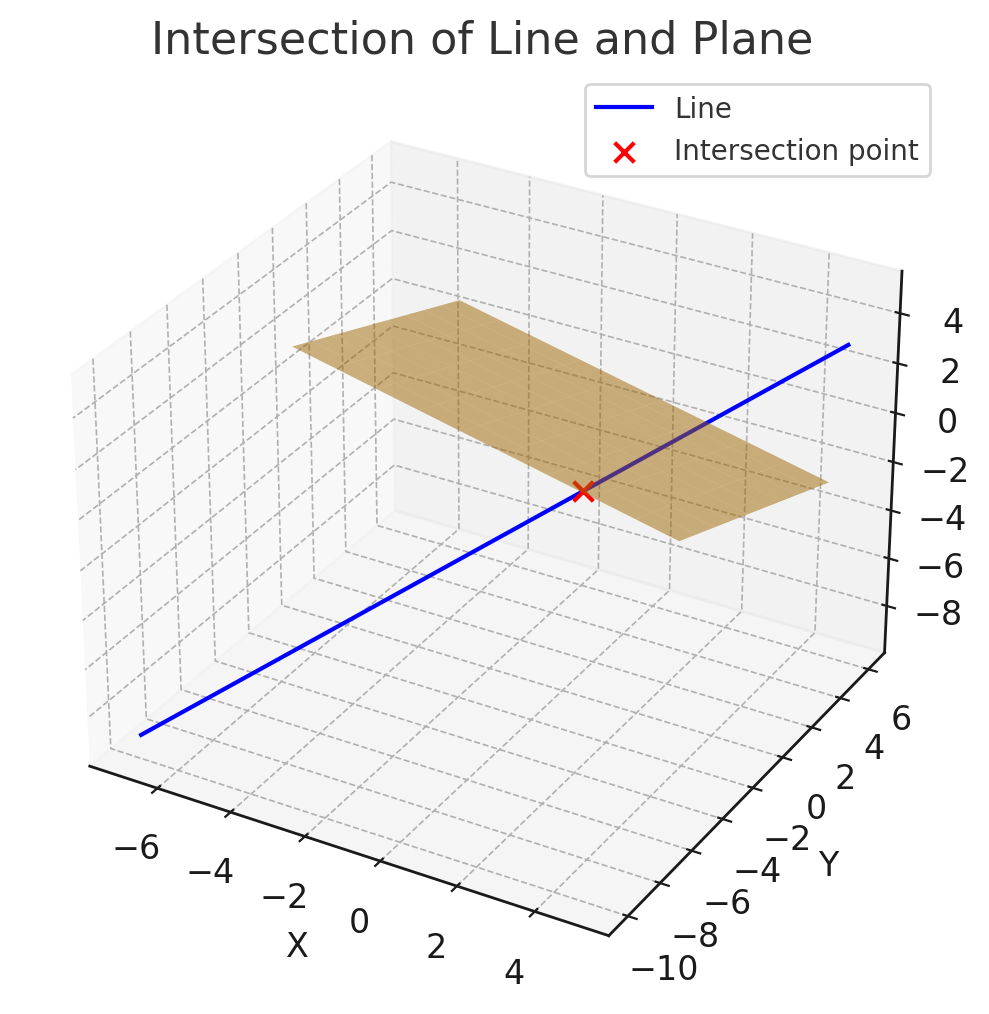
\includegraphics[width=\columnwidth, height=0.8\textheight, keepaspectratio]{beamer/figs/fig1.jpg}
   \label{fig:Beamer/figs/fig1.png}
\end{frame}

\end{document}
